\documentclass[a4paper]{article} 
\usepackage[14pt]{extsizes} % для того чтобы задать нестандартный 14-ый размер шрифта 
\usepackage[utf8]{inputenc} 
\usepackage[russian]{babel} 
\usepackage{amsmath,amsfonts,amssymb,amsthm,mathtools} 
\usepackage[left=20mm, top=15mm, right=15mm, bottom=15mm, nohead, footskip=10mm]{geometry} % настройки полей документа 

\begin{document} % начало документа 
% НАЧАЛО ТИТУЛЬНОГО ЛИСТА 
\begin{center} 
\hfill \break 
\large{Санкт-Петербургский Политехнический университет имени Петра Великого}\\ 
 
 \hfill \break 
\hfill\break 
\hfill \break 
\hfill \break 
\hfill \break 
\begin{center}\large{Отчёт по лабораторной работе №6} \end{center}  
\hfill \break 
\large{Тема:Решение задачи Коши для ОДУ} 
\hfill \break 
\hfill \break 
 
\hfill \break 
\hfill \break 
\\ 
\hfill \break 
\hfill \break 
\end{center} 


\normalsize{ 
\begin{tabular}{cccc} 
Студент & : & Алексеева Мария Сергеевна\\\\ 
Группа & : & 5030103/00003 \\\\ 
Преподаватель & : & Козлов Константин Николаевич \\\\ 
\end{tabular} 
}\\ 
\hfill \break 
\hfill \break 
\hfill \break 
\begin{center} Санкт-Петербург 2022 \end{center} 
\thispagestyle{empty} % выключаем отображение номера для этой страницы 
 
% КОНЕЦ ТИТУЛЬНОГО ЛИСТА 
\newpage 
	
\section{Формулировка задачи и её формализация} 
Задача: Решить ОДУ $y’=2x(x^2+y)$ на отрезке [1;2] при начальном условии y(a)=e методом Эйлера с итерационной обработкой. Исследовать изменение погрешности при различных факторах.Сравнить работу метода с методом Рунге-Кутты третьего порядка.
\section{Алгоритм метода и условия его применимости} 
\subsection{Алгоритм}
Для того, чтобы вычислить решение ОДУ методом Эйлера с пересчётом необходимо задать шаг, задается он по формуле $h=\dfrac{(b-a)}{n}$, где n количество разибений отрезка. Вычислив шаг, перейдем к заполнению массива узлов сетки: $x_i =x_0+h*i, i=1,2,3...; x_0=a, x_n=b$.
Далее с помощью начального условия зададим $y_0$ и заполним массив y. Зададим 4 "разгонные" точки. Для этого воспользуемся специальными формулами (для данного метода рекомендуется использовать не более трех-четырех приближений):\\
1)$y_k^0=y_{k-1}+hf(x_{k-1},y_{k-1})$ - для первой итерации\\
2) $y_k^{j+1}=y_{k-1}+\dfrac{h}{2}(f(x_{k-1},y_{k-1}+f(x_{k},y_{k}^{j}), j=0,1...$ - для последующих 3-ёх
3) Последнее значение запишем в массив Y. Цикл с итерациями повторяется от 1 до n. 

\subsection{Условия применимости}
На y' накладывается условие непрерывности за заданном отрезке, а также наличия интегральных кривых в любых точках.

 
\section{Предварительный анализ задачи} 
Ожидается, что при уменьшении шага мы будем наблюдать меньшую погрешность, как и для прошлых лабораторных. При внесении возмущений в различные данные мы будем получать увеличение ошибки, но сложно предположить его величину. 
\section{Тестовый пример с расчётами} 
В качестве примера рассмотрим простой диффур $y'=y/x$ с задачей Коши y(1) = 1. Точное решение y=x. Решим задачу на отрезке [1;2].Будем решать с двумя итерационными приближениями.\\
1)Зададим n=2, получим шаг 0.5\\
2)$x_0= 1$ $x_1=1.5$  $x_2=2$\\
3)$y_0=1$\\
Вычислим $y_1$:\\
$y_1^0=y_0+hf(x_0,y_0)=1+0.5\dfrac{1}{1}=1.5$\\
$y_1^1=+y_0+\dfrac{h}{2}(f(x_0,y_0)+f(x_1,y_1^0))=1+\dfrac{0.5}{2}(\dfrac{1}{1}+\dfrac{1.5}{1.5})=1.5$\\
$y_1=1.5$
Вычислим $y_2$:\\
$y_2^0=y_1+hf(x_1,y_1)=1.5+0.5\dfrac{1.5}{1.5}=2$\\
$y_2^1=y_1+\dfrac{h}{2}(f(x_1,y_1)+f(x_2,y_2^0))=1.5+\dfrac{0.5}{2}(\dfrac{1.5}{1.5}+\dfrac{2}{2})=2$\\
$y_2=2$ \\
Получили массивы X = [1; 1.5; 2] Y = [1;1.5;2], как несложно заметить имеем совпадение с точным решением.

 
\section{Подготовка контрольных тестов для иллюстрации метода} 

Решение ОДУ будем искать на отрезке [1;2]. В качестве первого исследования мы посмотрим на погрешность при шаге h=0.01, затем проверим, как меняется погрешность от изменения шага от 0.1 до 0.0001. Далее рассмотрим ситуацию внесения возмущения 1,2 и 3 процента в числовые коэффициенты, в моем случае это будет возмущение d: 
$y = 2x(d \times x^2+y)$. В результатах исследования укажем относительную погрешность. Далее вносить такие же возмущения будем в начальные данные и соответственно также в результате получим относительные погрешности для трех случаев. Все эти исследования мы получим и для метода Рунге-Кутты третьего порядка, сравним их с методом Эйлера с итерационной обработкой. Последние исследования будут связаны с правилом Рунге для метода Эйлера. Построим график с теоретической и фактической точностью, полученной при вычислениях и посмотрим какой шаг необходим для заданной точности. \\

\newpage
\section{Модульная структура программы} 
 
\begin{figure}[h!]
\begin{center}
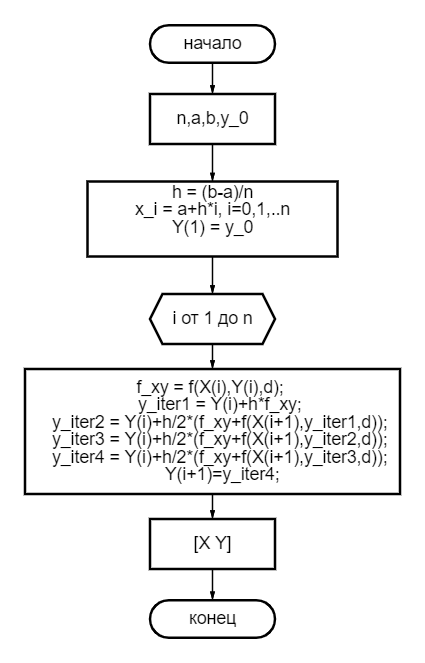
\includegraphics[scale=0.7]{diagram (6).png} 
\end{center}
\caption{Блок-схема метода Эйлера с итерационной обработкой} \label{Рис1}
\end{figure}

\begin{figure}[h!]
\begin{center}
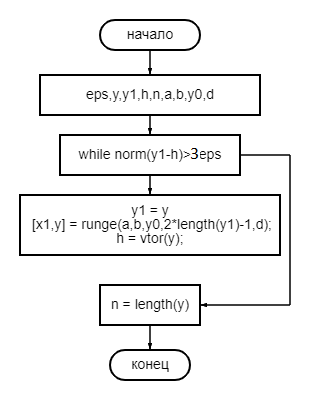
\includegraphics[scale=0.7]{diagram (6)1.png} 
\end{center}
\caption{Блок-схема правила Рунге} \label{Рис2}
\end{figure}

\newpage
\section{Численный анализ решения задачи}

\begin{figure}[h!]
\begin{center}
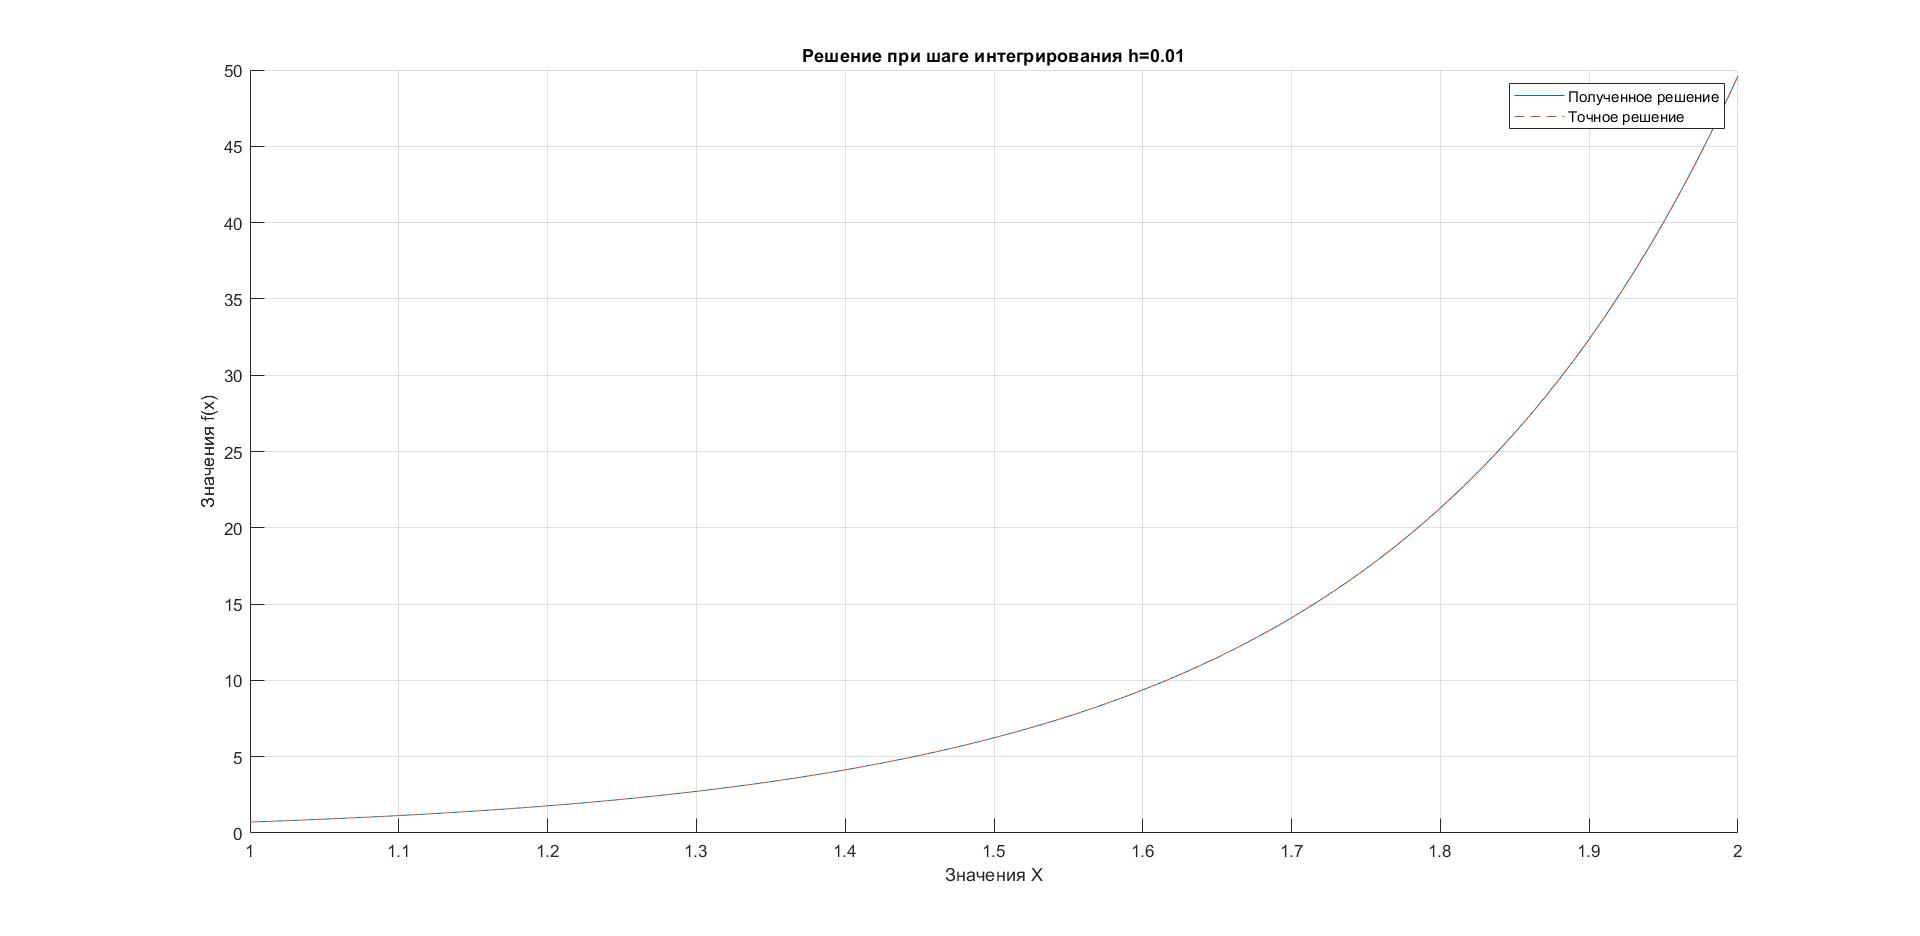
\includegraphics[scale=0.3]{решение при шаге 0.01.jpg} 
\end{center}
\caption{Решение при шаге 0.01} \label{Рис3}
\end{figure}

\begin{figure}[h!]
\begin{center}
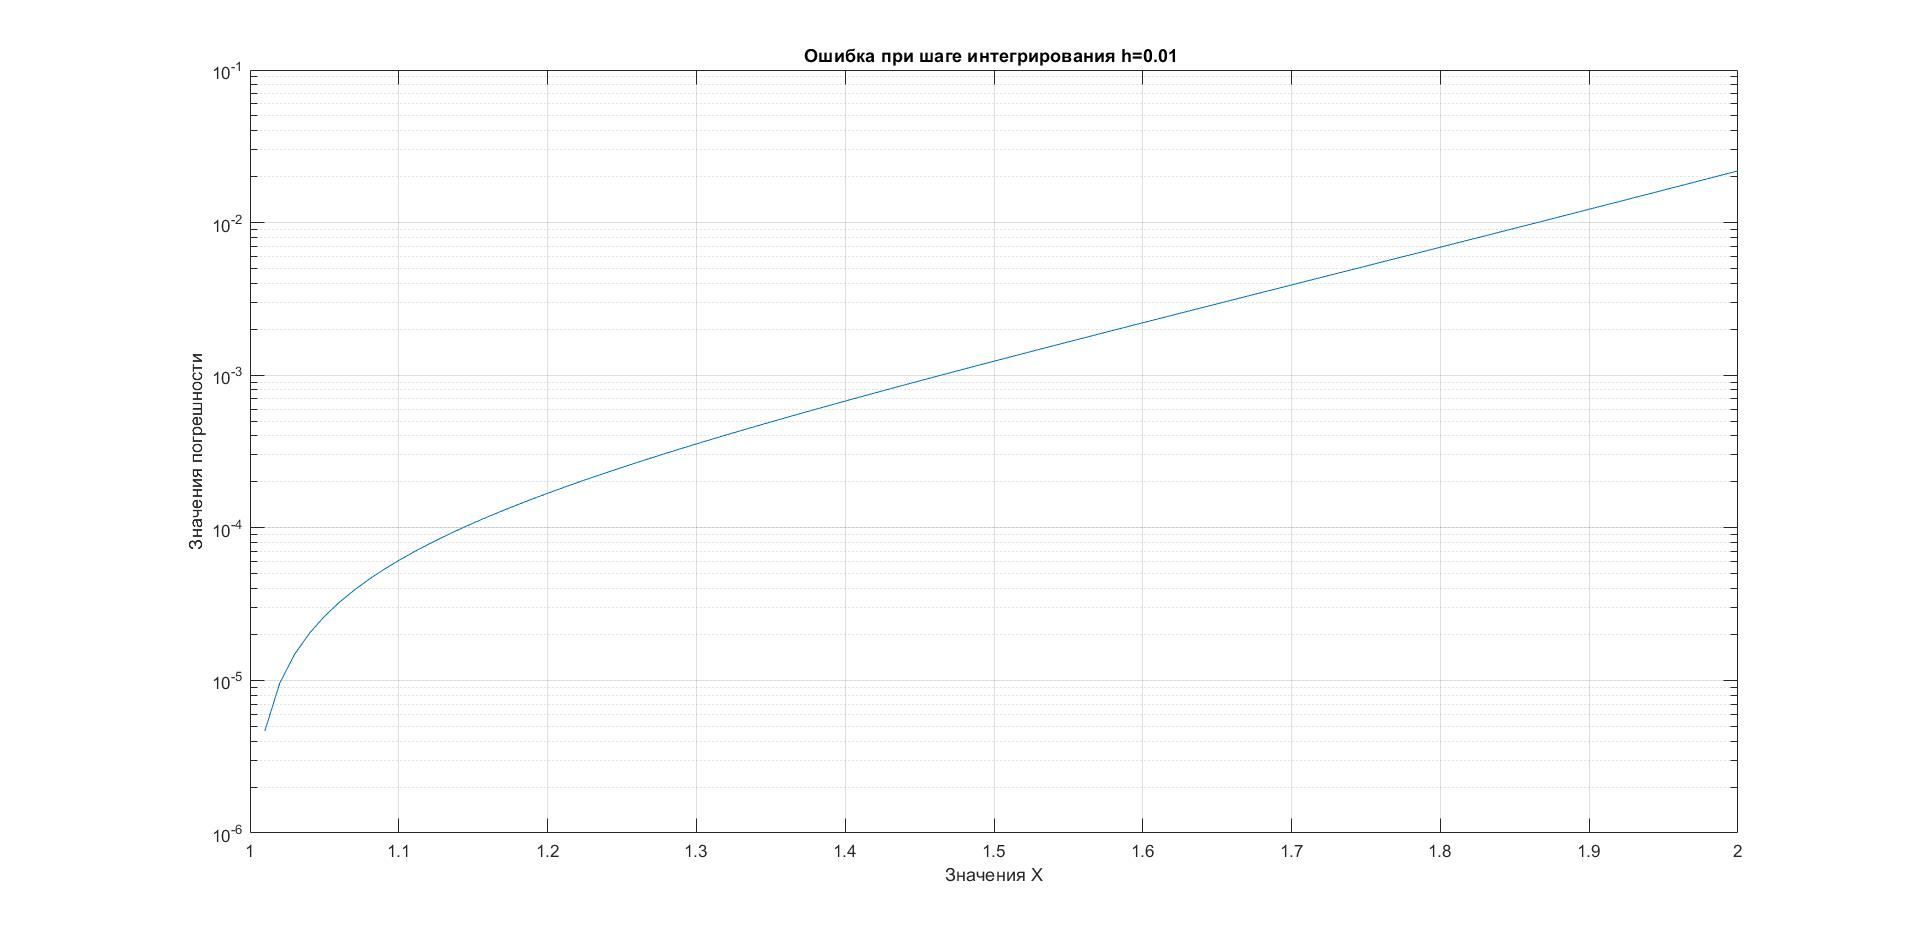
\includegraphics[scale=0.3]{ошибка при шаге 0.01.jpg} 
\end{center}
\caption{Ошибка при шаге 0.01} \label{Рис4}
\end{figure}
Перед тем, как проводить исследования проверим порядок точности. Переменная poryadok=2, что говорит о том, что порядок точности равен двум. Теперь перейдём к исследованиям.
Для начала хотелось бы представить график решения ОДУ при шаге 0.01. Как можно увидеть из рисунка \ref{Рис3} решение получается точным, но стоит всё же обратиться к отдельному графику погрешности для того же фиксированного шага. Для этого обратим внимание на график на рисунке \ref{Рис4} как видим, в начале отрезка меньшая погрешность около $10^{-5}$,она возрастает к его концу до $10^{-3}$.



\subsection{Исследование зависимости погрешности от изменения различных данных} 

\begin{figure}[h!]
\begin{center}
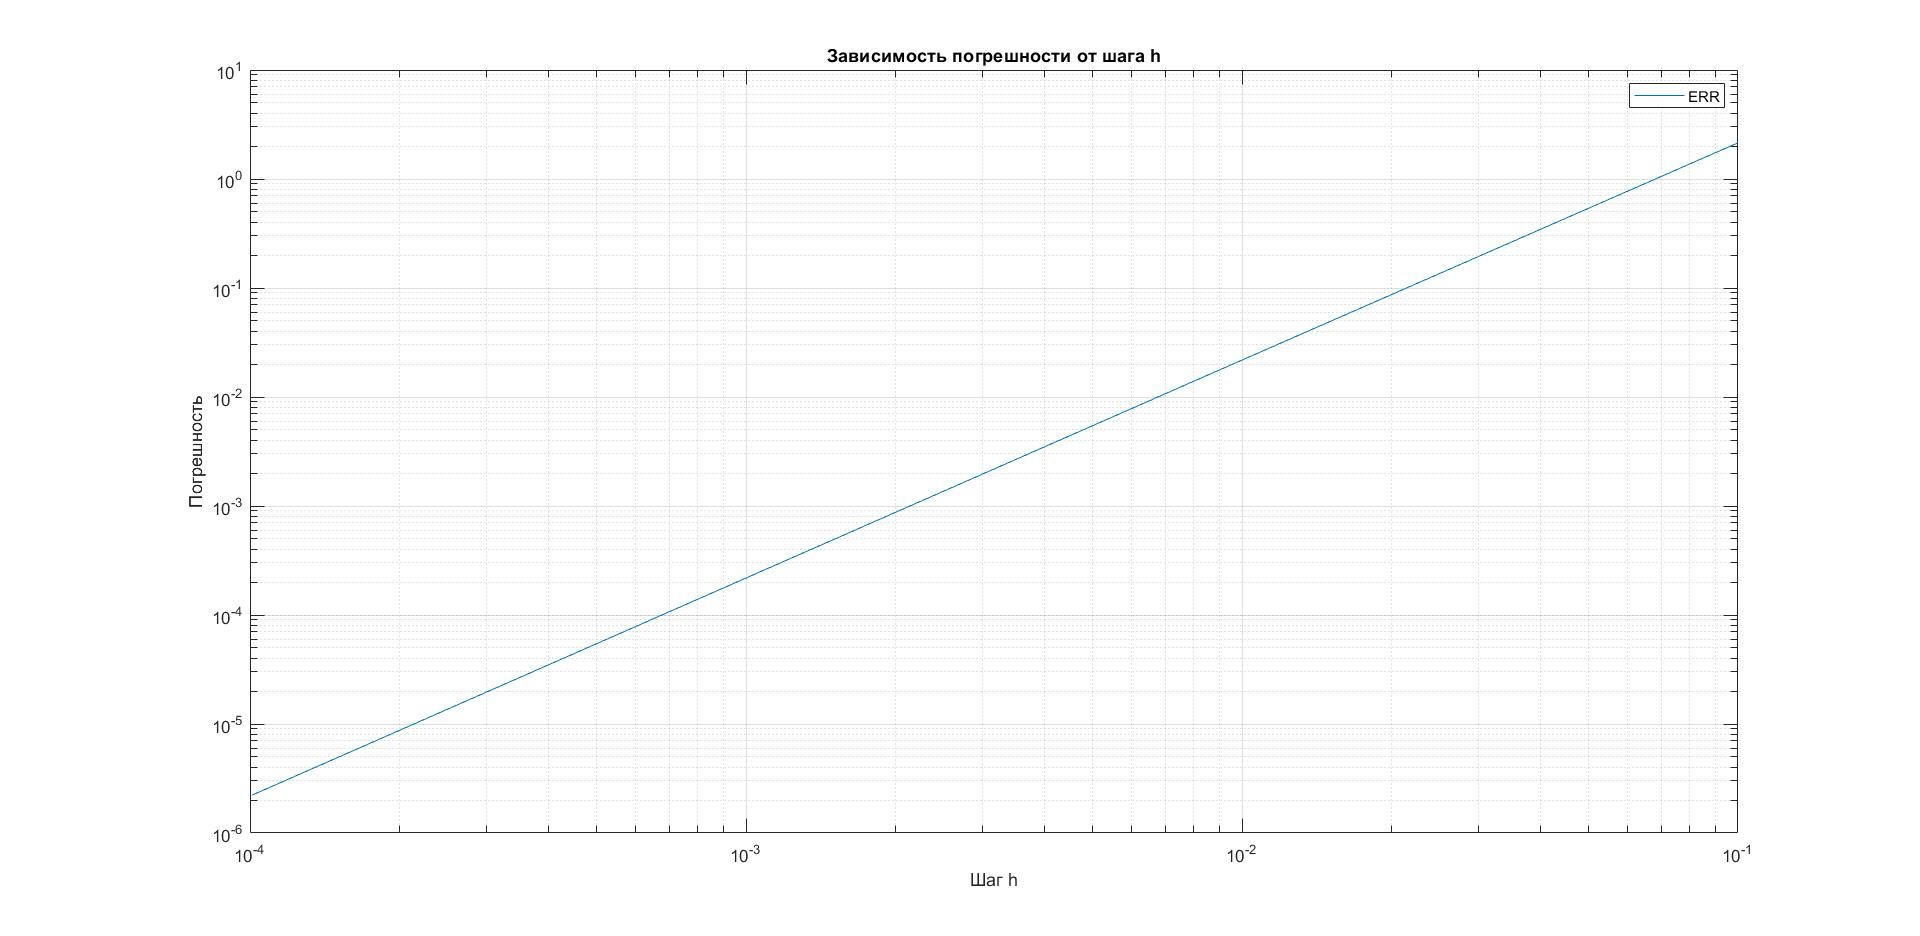
\includegraphics[scale=0.3]{погрешность от шага.jpg} 
\end{center}
\caption{Зависимость погрешности от шага} \label{Рис5}
\end{figure}
Теперь обратимся к исследованию зависимости погрешности ошибки от шага. На рисунке $\ref{Рис5}$ изображен график по оси абсцисс которого отмечается шаг h, по оси ординат максимальная погрешнось при заданном шаге.Шаг меняется от 0.1 до 0.0001, как несложно заметить,чем больше шаг, тем больше погрешность. 


\begin{figure}[h!]
\begin{center}
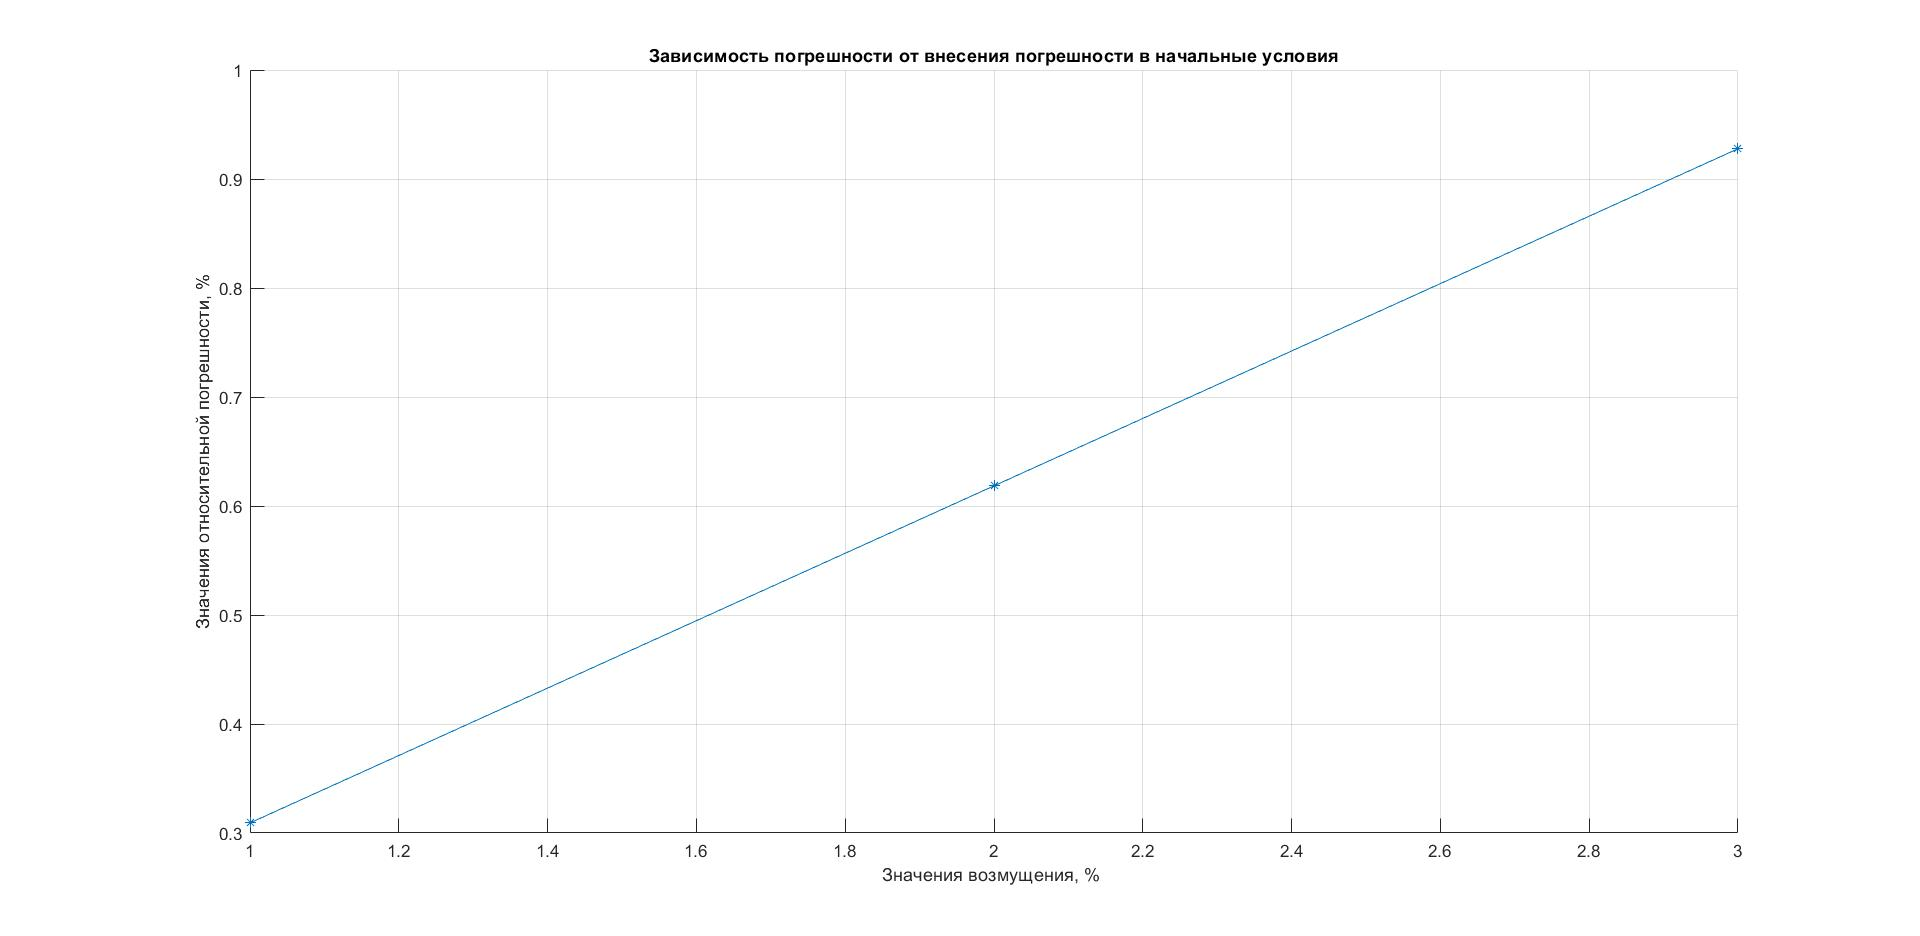
\includegraphics[scale=0.3]{возмущение в начальные условия.jpg}  
\end{center}
\caption{Зависимость погрешности от внесения возмущения в начальные условия} \label{Рис6}
\end{figure}

\begin{figure}[h!]
\begin{center}
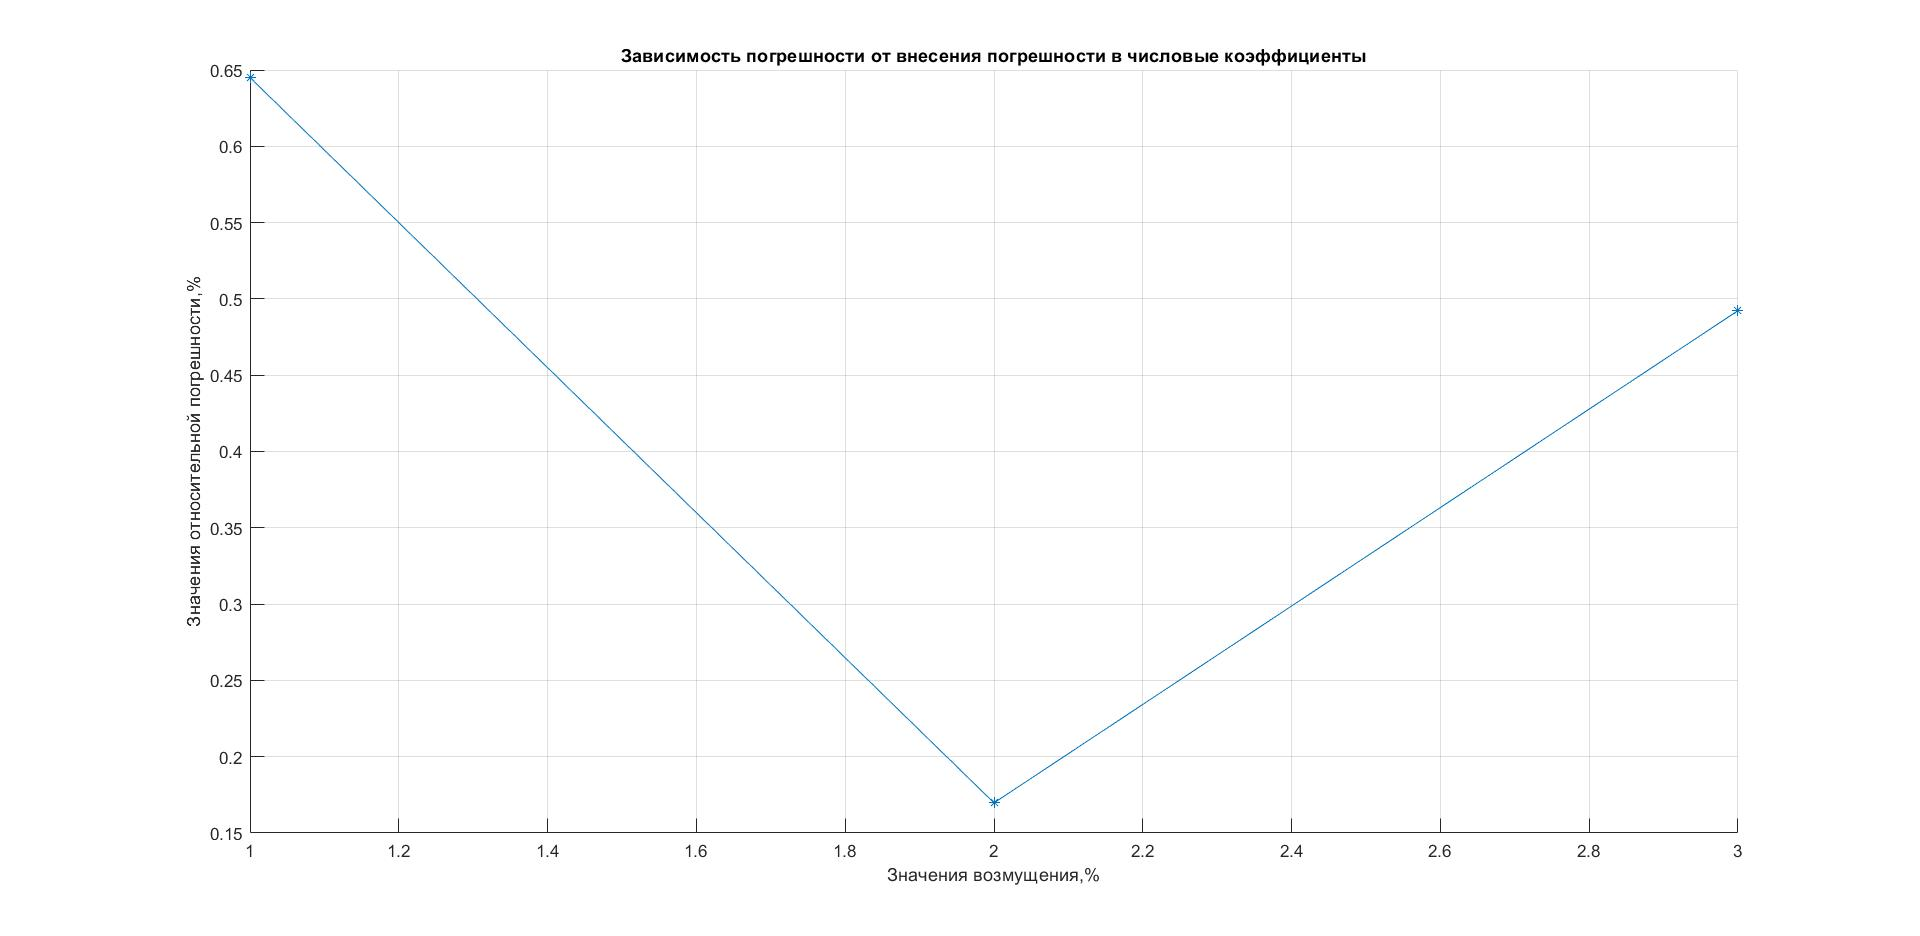
\includegraphics[scale=0.3]{возмущение в числовые коэффициенты.jpg} 
\end{center}
\caption{Зависимость погрешности от внесения возмущения в числовые коэффициенты} \label{Рис7}
\end{figure}
Далее рассмотрим, как ведет себя погрешность при возмущении некоторых данных. Посмотрим на графики на рисунках $\ref{Рис6}$ и $\ref{Рис7}  $. По оси абсцисс будем отмечать возмущение в процентах, по оси ординат отметим относительную ошибку в процентах. Возмущения для двух случаев вносились разными способами. Для начальных условий мы просто увеличиваем $y_0$ на определенный процент. Для числовых коэффициентов бралось возмущения пределах определенного процента, т.е., если возмущение на графике 1 процент, то имеет числов пределах [-1;1], таким же образом и для 2-ух и 3-ёх процентов. На графике рисунка \ref{Рис6} изображена погрешность полученная при внесении возмущения в начальные условия, как можем заметить процент ошибки достаточно мал, на рисунке \ref{Рис7} отмечена относительная погрешность, полученная при внесении возмущения в числовые коэффициенты, здесь процент ошибки также мал.

\subsection{Исследования, связанные с правилом Рунге} 

\begin{figure}[h!]
\begin{center}
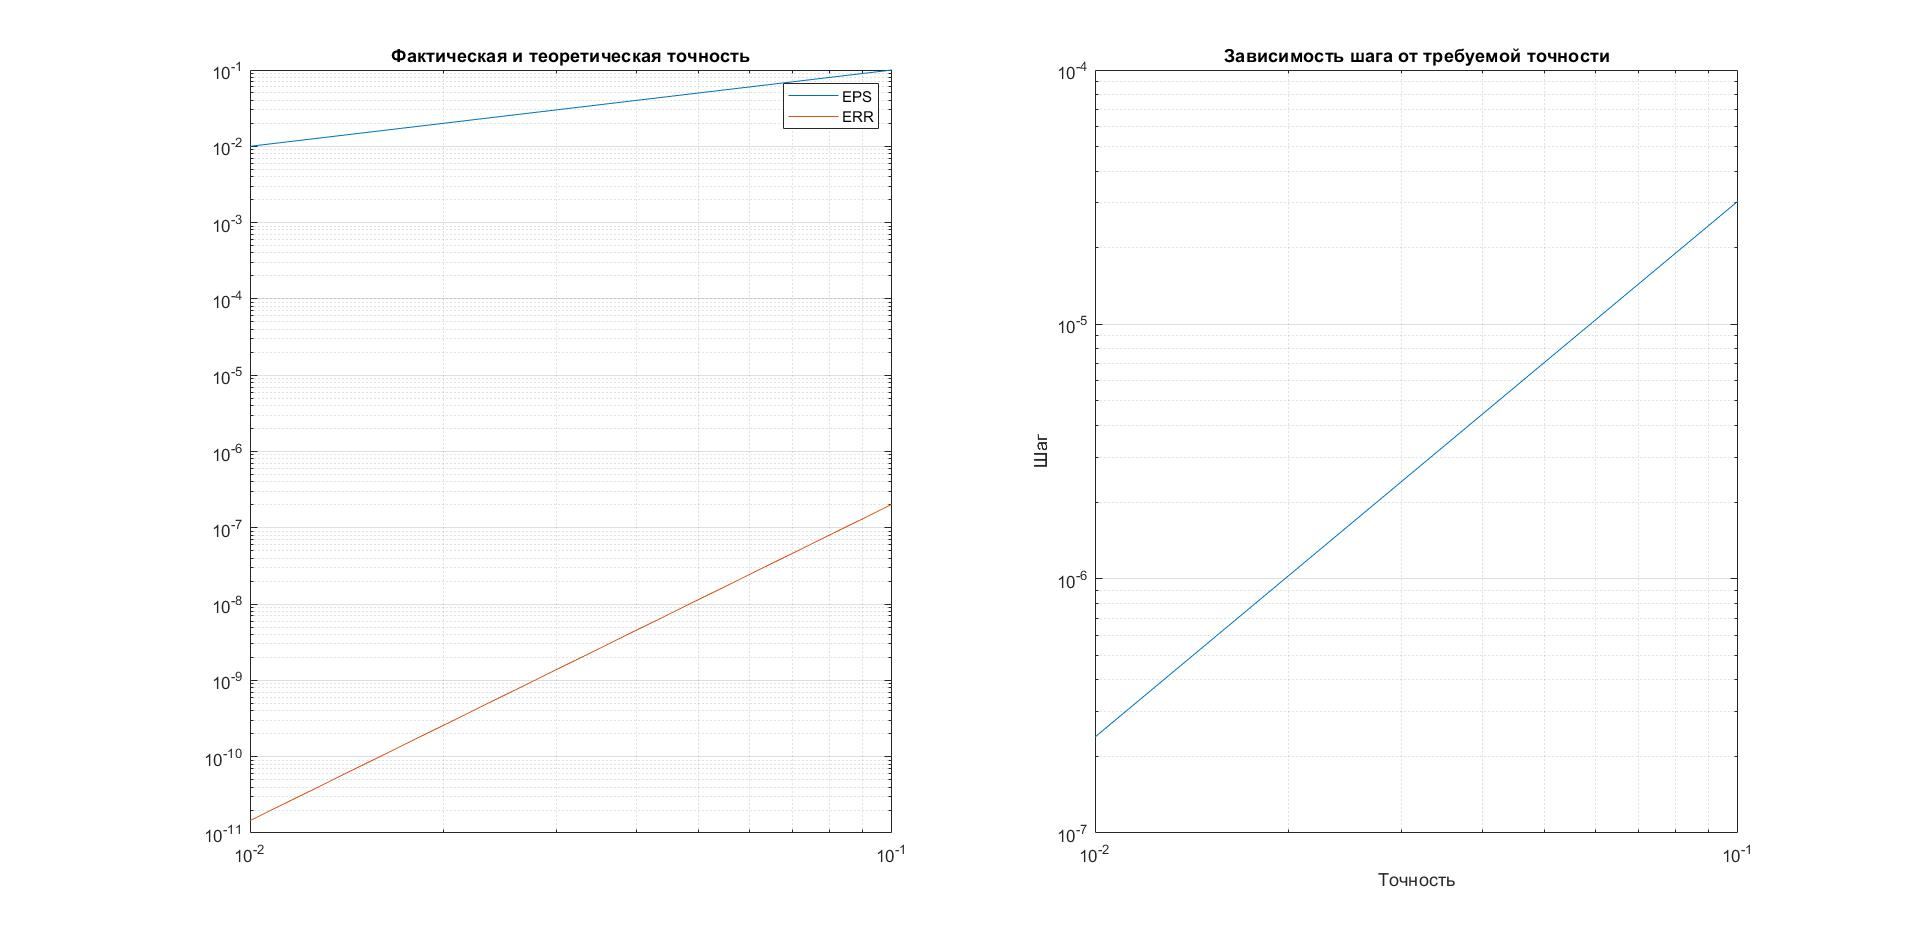
\includegraphics[scale=0.3]{правило рунге.jpg} 
\end{center}
\caption{Графики, полученные с использованием правила Рунге} \label{Рис8}
\end{figure}
На первом графике на рисунке $\ref{Рис8}$ можно отметить, что фактическая точность не превышает теоретической, что и ожидалось.Провести исследование получается только до требуемой точности равной $10^{-2}$. Далее проверить не позволяет программа, но даже при таком исследовании можно наблюдать, что точность достаточно хороша.  На втором графике того же рисунка мы видим, какой шаг необходимо использовать для получения нужной точности. Как можно заметить, чем меньший шаг мы берем, тем более "хорошее" значение точности мы получаем. Можно увидеть, что для "хорошей" точности нужно брать достаточно маленький шаг, так для точности $10^{-2}$ шаг должен быть $10^{-7}$.\\


\newpage
\section{Сравнение исследований для двух методов}

\begin{figure}[h!]
\begin{center}
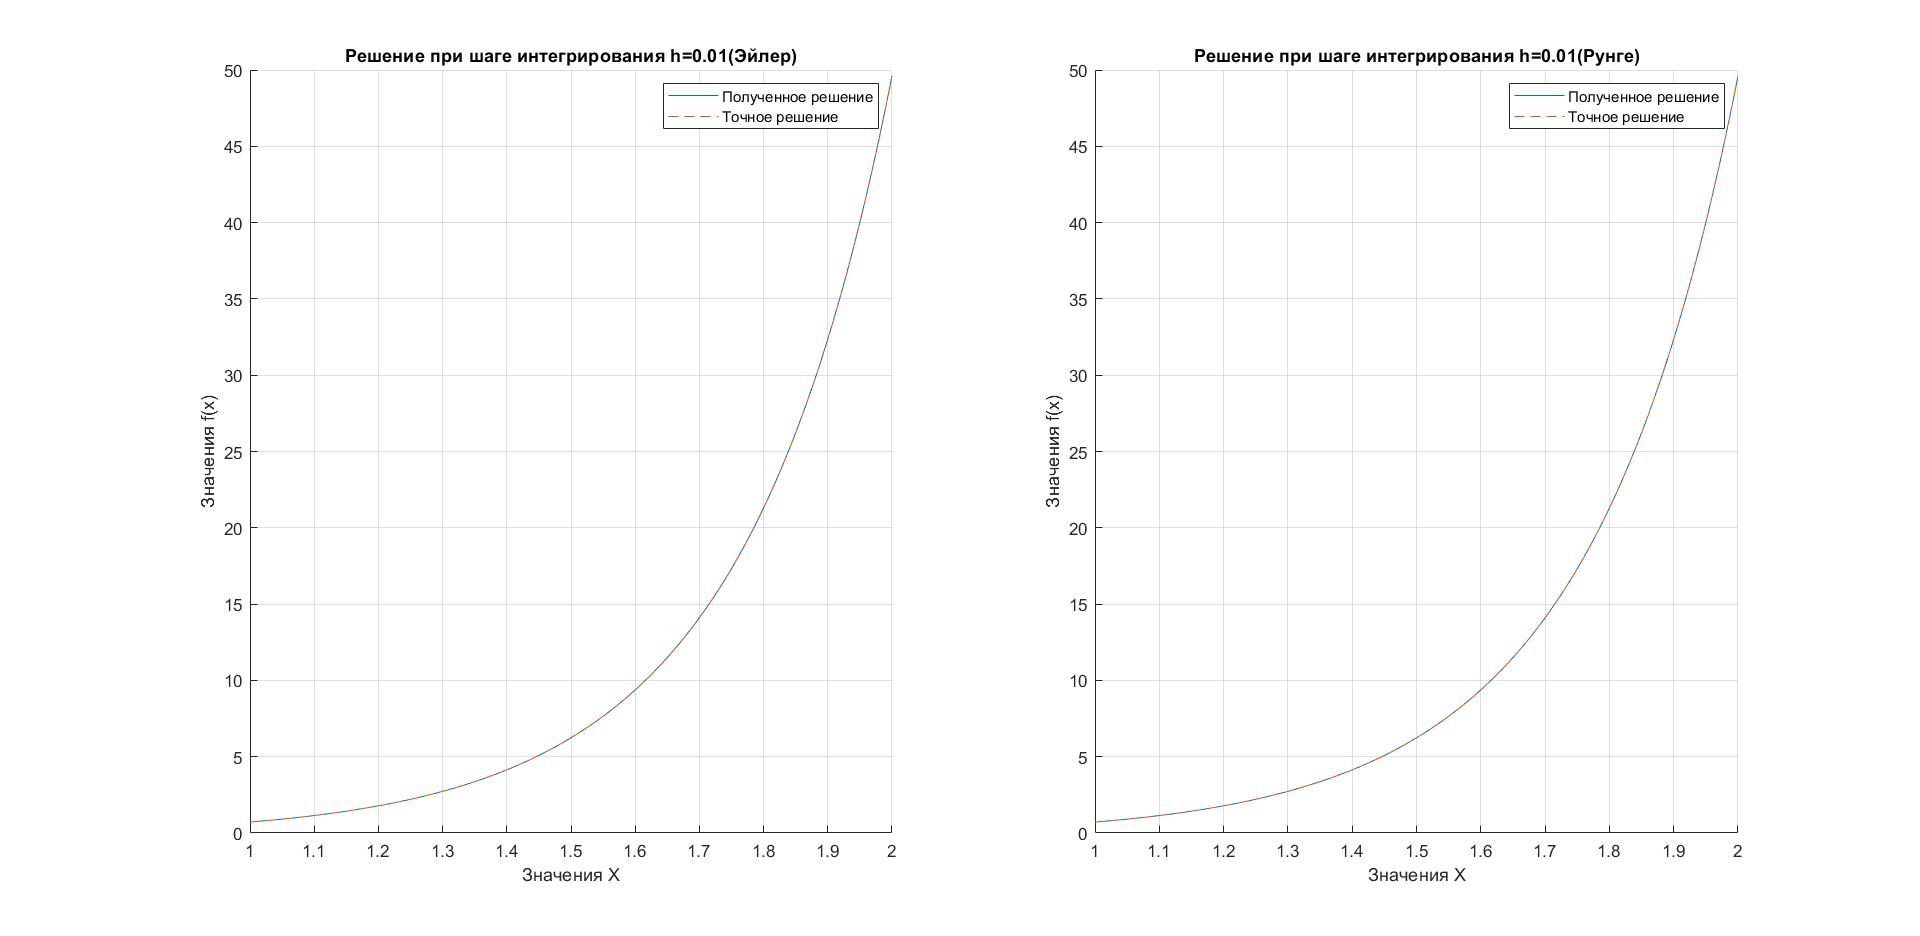
\includegraphics[scale=0.3]{сравнение решение.jpg} 
\end{center}
\caption{Сравнение решений} \label{Рис9}
\end{figure}

\begin{figure}[h!]
\begin{center}
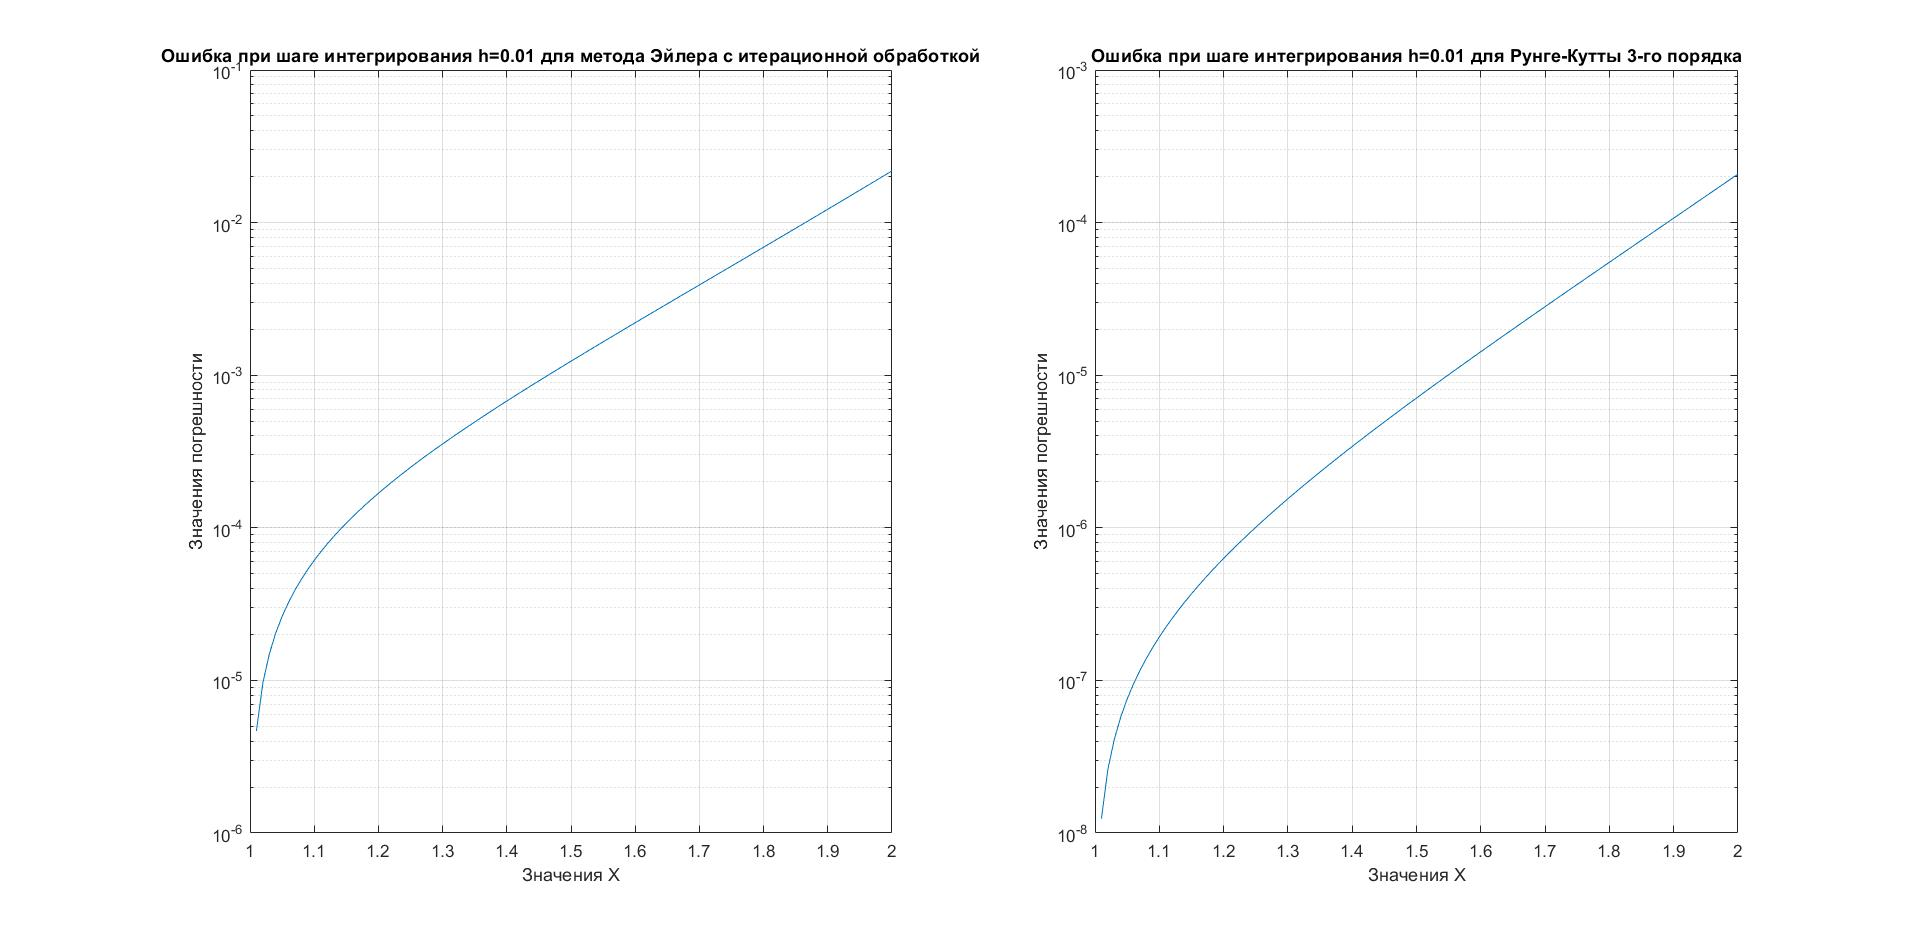
\includegraphics[scale=0.3]{сравнение ошибка при шаге.jpg} 
\end{center}
\caption{Сравнение погрешности при шаге 0.01} \label{Рис10}
\end{figure}

Обратимся к графику на рисунке $\ref{Рис9}$. На первый взгляд может показаться, что решения для двух методов точны и почти одинаковы между собой. Но, чтобы точно разобраться, стоит обратиться к графикам погрешностей. Посмотрим на рисунок $\ref{Рис10}$, как можно заметить погрешность метода Эйлера с пересчётом на порядки больше, чем для метода Рунге-Кутты третьего порядка. В точке 1 метод Эйлер даёт погрешность около $10^{-5}$, метод Рунге-Кутты - ближе к $10^{-8}$. Почти аналогичную ситуацию можно наблюдать на всём отрезке, меняются погрешности, но их разница остается примерно одинакова. 

\begin{figure}[h!]
\begin{center}
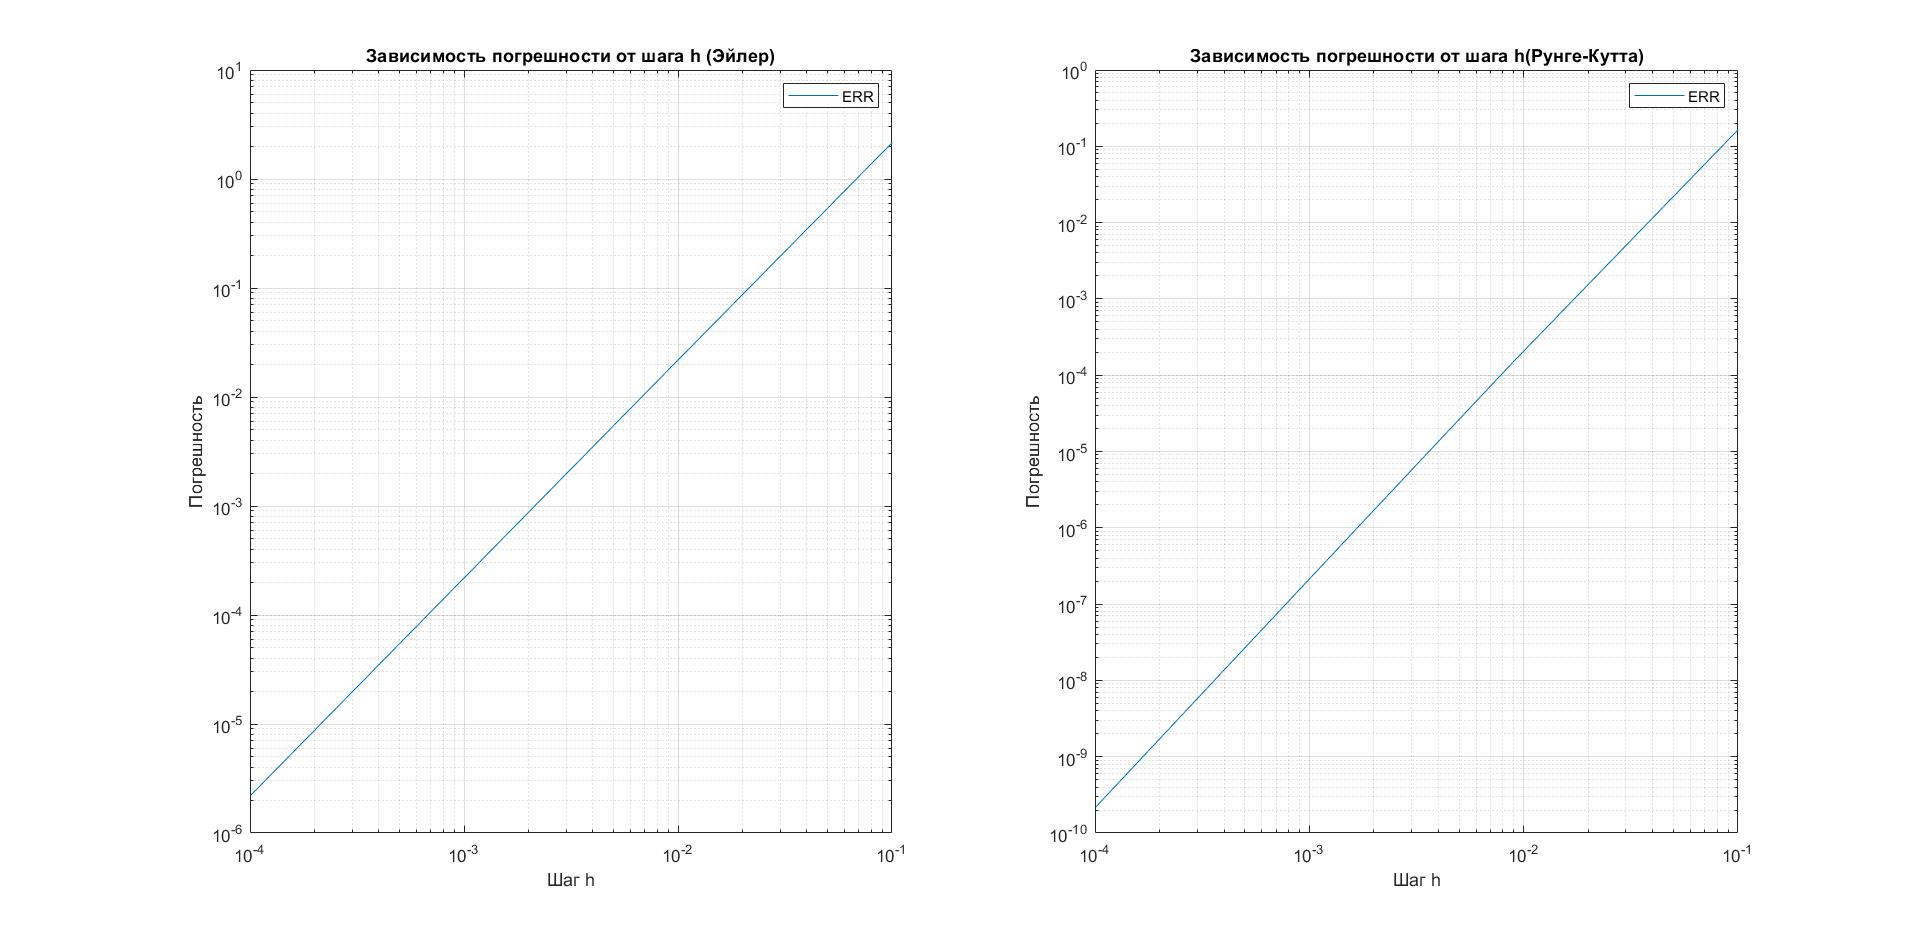
\includegraphics[scale=0.3]{сравнение от шага.jpg} 
\end{center}
\caption{Сравнение погрешности в зависимости от шага h} \label{Рис11}
\end{figure}
Чтобы более подробно сравнить погрешности двух методов, обратимся к рисунку $\ref{Рис11}$. Посмотрим, как меняется погрешность двух методов при меняющемся шаге. Как можно заметить метод Эйлера даёт большую погрешность, чем метод Рунге-Кутты.

\begin{figure}[h!]
\begin{center}
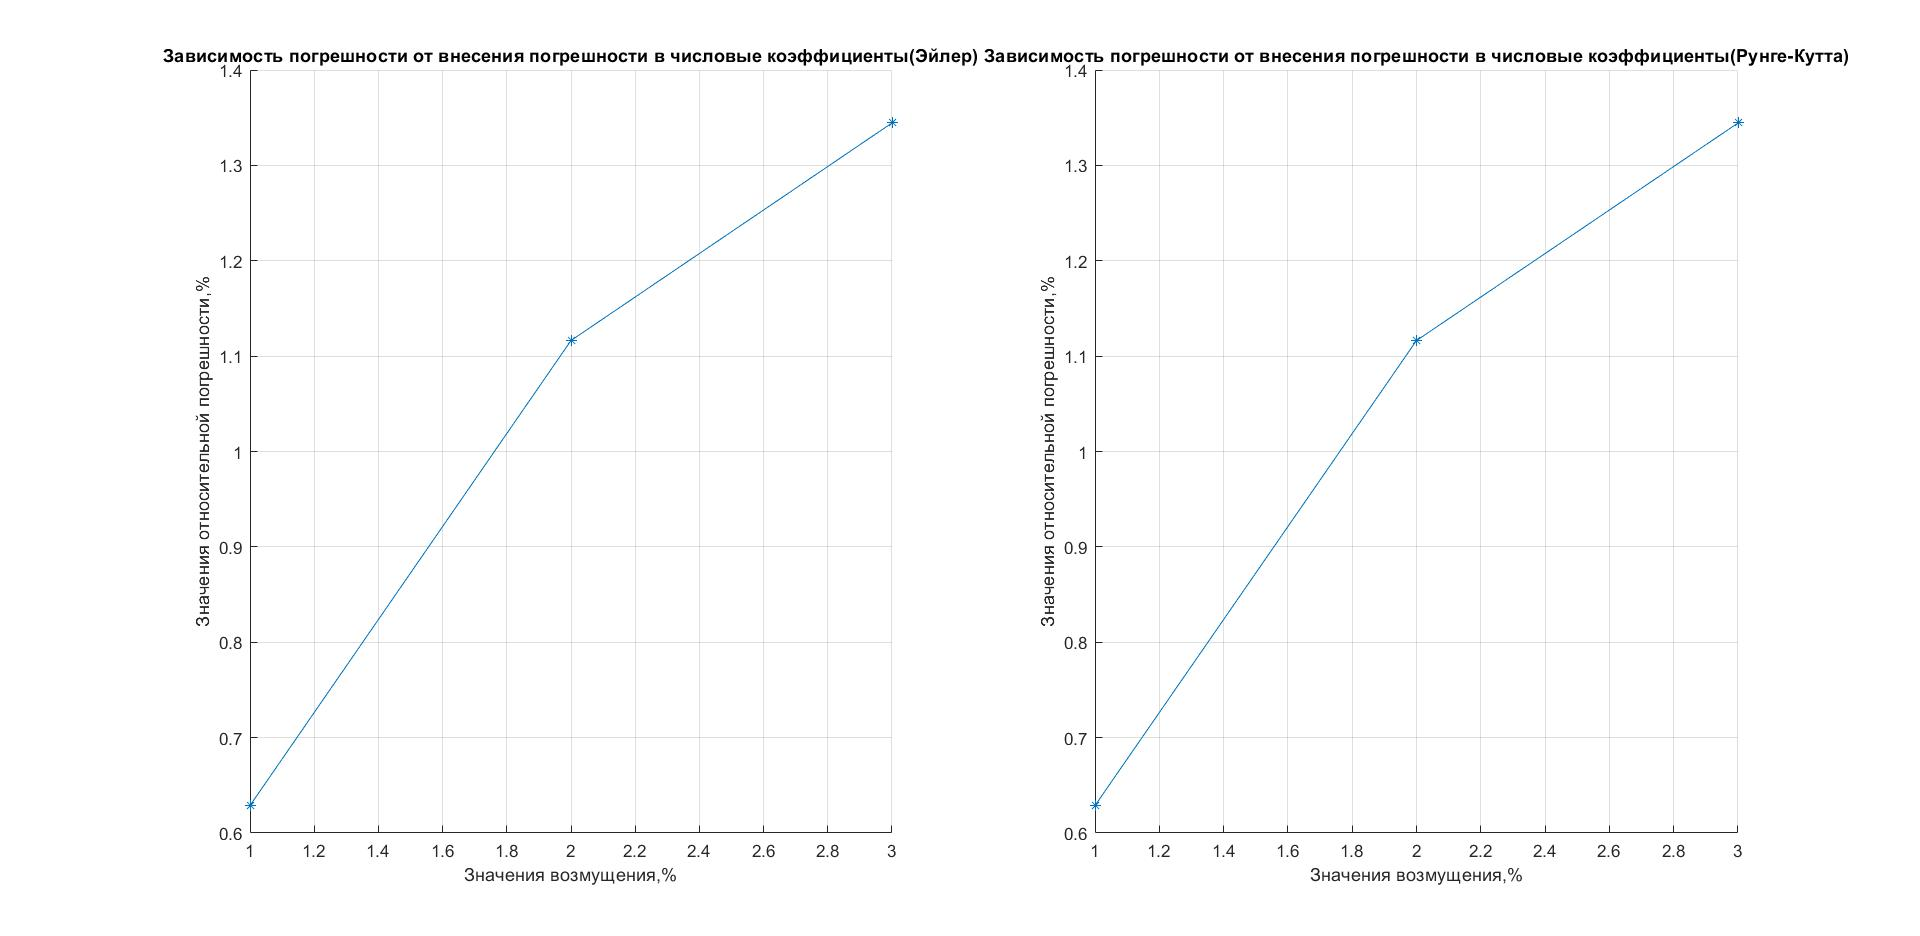
\includegraphics[scale=0.3]{сравнение возмущение коэф.jpg} 
\end{center}
\caption{Сравнение погрешности в зависимости от возмущени в коэффициентах} \label{Рис12}
\end{figure}

\begin{figure}[h!]
\begin{center}
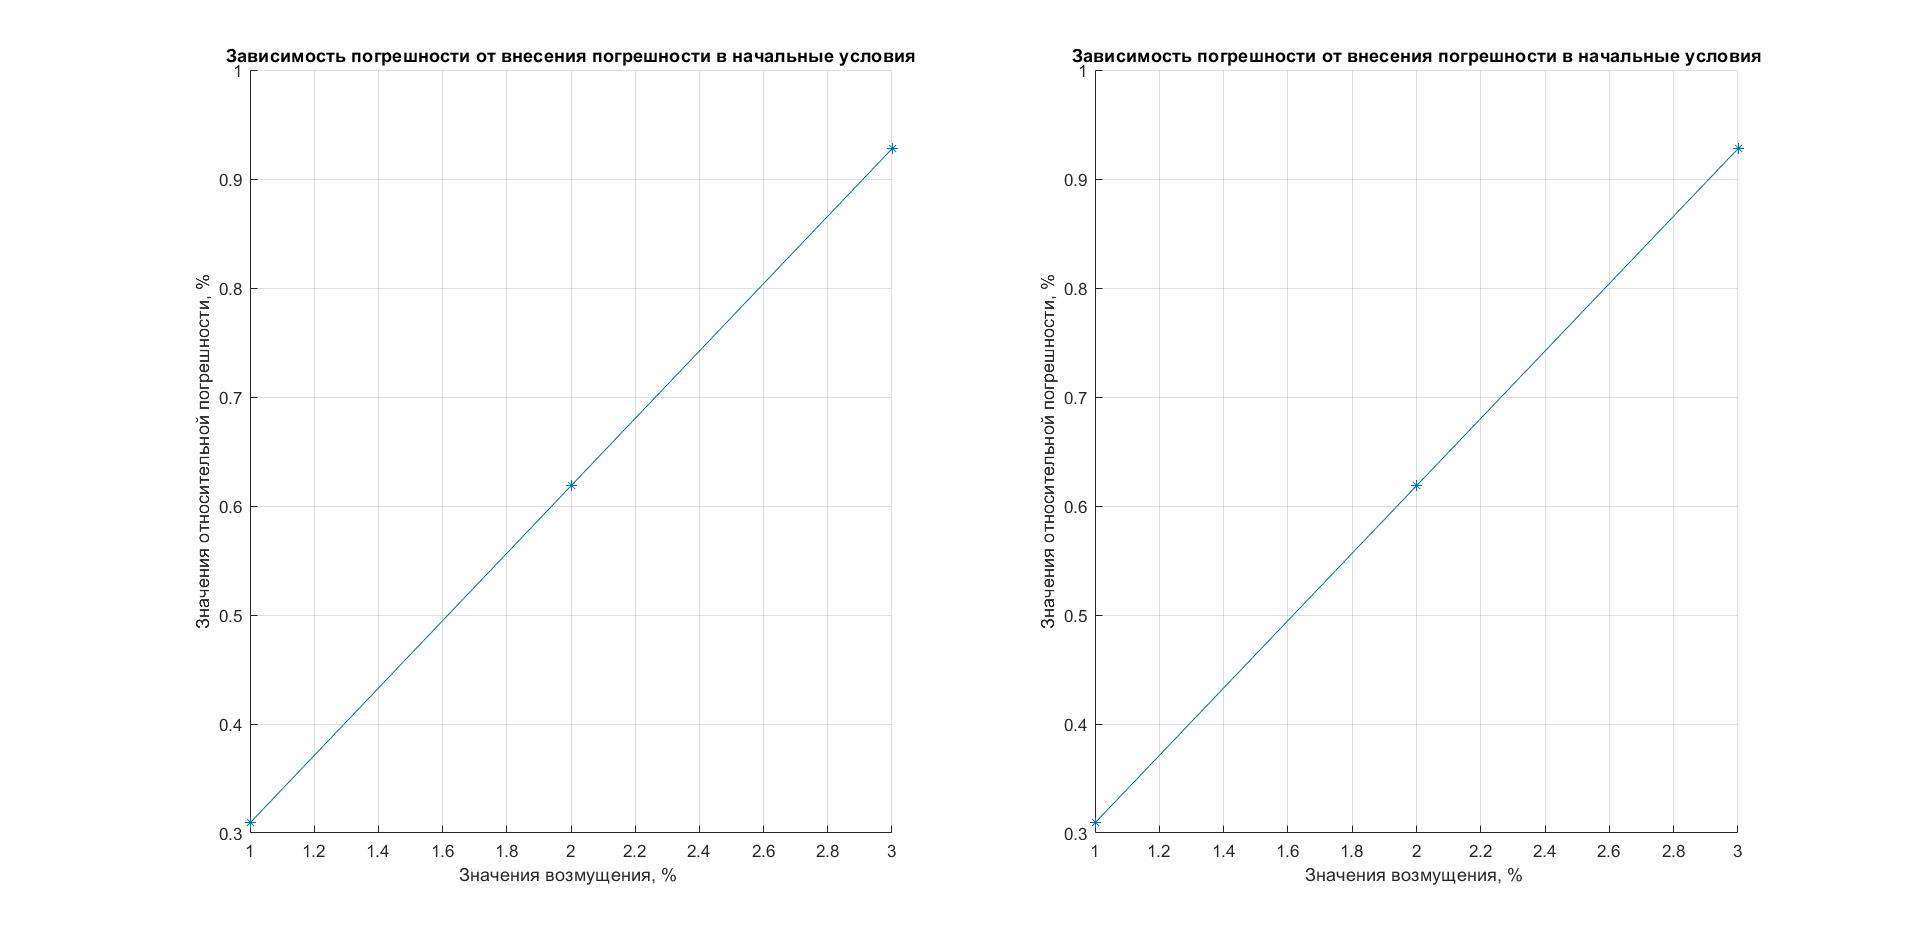
\includegraphics[scale=0.3]{сравнение возмущение нач усл.jpg} 
\end{center}
\caption{Сравнение погрешности в зависимости от возмущени в начальных условиях} \label{Рис13}
\end{figure}
Обратимся к последним исследованиям, а именно влияние возмущения на погрешность для двух методов.На рисунках $\ref{Рис12}$ и $\ref{Рис13}$ можем наблюдать, что процент погрешности, что у метода Эйлера, что у метода Рунге-Кутты примерно одинаков. 



\newpage
\section{Краткие выводы} 

\begin{itemize}
  \item Метод Эйлера с пересчётом дает достаточно точные результаты, если взять достаточно маленький шаг.
  \item Все исследования удовлетворили предварительному анализу.
  \item Можно заметить, что метод является достаточно устойчивым, потому что вносимые возмущения не дали большую погрешность. При этом метод Эйлера так же устойчив, как и метод Рунге-Кутты
  \item При сравнении метода Эйлера с итерационной обработкой и метода Рунге-Кутты 3-го порядка можно наблюдать, что погрешности при разных исследованияъ у метода Эйлера с пересчётом получались больше, чем у Рунге-Кутты. Это оправдывается тем, что порядок точности у метода Эйлера меньше. 
  \end{itemize}


\end{document} % КОНЕЦ ДОКУМЕНТА !

